\documentclass[times,twocolumn,final,authoryear]{elsarticle}
\usepackage{vendor/prletters}
\usepackage{amsmath,amssymb,booktabs,graphicx,url}
\usepackage[hidelinks]{hyperref}
% Draft-only front matter overrides for the licensed 2013 PRL template.
% Body geometry, font size, column widths, caption style remain from prletters.
% Do not print fictitious publisher copyright, receipt dates, or publisher logo.
\makeatletter
\def\ps@PRlettersTitle{\def\@oddhead{\small Pattern Recognition Letters\hfill Research manuscript\quad\thepage}\let\@evenhead\@oddhead\def\@oddfoot{}\let\@evenfoot\@oddfoot}
\renewenvironment{abstract}{\global\setbox\absbox=\vbox\bgroup\hsize=\textwidth\noindent\textbf{Abstract}\par\small\noindent}{\par\egroup}
\def\keyword{\global\setbox\keybox=\vbox\bgroup\hsize=\textwidth\small\noindent\textit{Keywords: }\def\sep{;\space}\ignorespaces}
\def\endkeyword{\par\egroup}
\long\def\MaketitleBox{\resetTitleCounters\begin{flushleft}\Large\bfseries\@title\par\vskip12pt\normalfont\small\elsauthors\par\vskip12pt\unvbox\absbox\vskip8pt\unvbox\keybox\end{flushleft}\vskip12pt}
\makeatother

\journal{Pattern Recognition Letters}
\graphicspath{{figures/}}
\makeatletter
\let\tableinput\@@input
\makeatother
\begin{document}
\begin{frontmatter}
\title{Selective mask readout calibration through predicted correction benefit}
\author{Research manuscript; author information supplied separately}
\begin{abstract}
Prototype-based instance segmentation converts continuous mask logits into binary predictions. Tightening this readout can remove excess foreground, but also damages correctly segmented instances. We study this trade-off with frozen detections and propose response-conditioned mask calibration (RCMC). A small regressor predicts the IoU change caused by a trial tightening from mask geometry and the fraction of foreground it removes. The original mask is retained when the predicted benefit is nonpositive. On 4,500 COCO validation images, RCMC raises YOLO26m-seg mask AP from 43.38 to 43.94, with gains of 0.78 AP$_{75}$ and 0.88 AP$_S$. A gate fitted on m-model training predictions transfers to YOLO26s-seg without refitting, improving mask AP by 0.47 points. Relative to uniform application of the same tightening, the gate reduces previously correct instances damaged at IoU 0.75 by 23\% and 30\%, respectively. Boundary-only and filtering-only controls attribute nearly all of the fixed intervention's AP gain to changed masks. These results identify a correctable readout failure and demonstrate selective repair using existing predictions. Evaluation remains within one architecture family, and the current gate adds measurable inference cost.
\end{abstract}
\begin{keyword}
Instance segmentation \sep Mask calibration \sep Error diagnosis \sep Boundary correction
\end{keyword}
\end{frontmatter}

\section{Introduction}
Instance segmentation systems must decide whether to retain an object hypothesis and which pixels to assign to it. A correctly localized candidate can still fail a strict mask-overlap criterion. Such predictions offer a useful diagnostic starting point: the object has already been found, yet its recovered foreground is inaccurate. Mask quality scoring and boundary refinement address related aspects of this problem \citep{huang2019maskscoring,kirillov2020pointrend,tang2021bpr}. We investigate whether the response of an existing mask to a simple tightening operation contains enough information to decide when that operation should be applied.

Prototype-based decoders combine shared spatial prototypes with instance coefficients \citep{bolya2019yolact}. Their binary readout introduces a decision boundary within an already computed logit map. Raising its threshold suppresses weak positive responses, including both erroneous exterior pixels and valid foreground. A trial tightening can consequently help one instance and harm another. An aggregate AP gain alone does not reveal this conflict, nor does observing excess foreground establish which upstream network component produced it.

We start from a specific failure: a candidate has a good box and covers almost all of its target, but its mask IoU is low. For this object, adding foreground is unlikely to be the most useful action. A controlled readout intervention can test whether its existing logits already permit a better foreground--background trade-off. If useful corrections coexist with substantial damage to correct masks, the next question becomes how to select the intervention using predictions alone.

Our contribution is a controlled diagnosis and a selective correction rule. We isolate mask readout by holding logits, boxes, categories, confidence scores, and candidate identity fixed; learn the continuous IoU benefit of a fixed intervention from prediction-derived features; and evaluate both aggregate performance and the instances repaired or damaged. The gate uses baseline-mask geometry and a response feature: how much foreground the trial removes. It observes no test annotations and requires no segmenter retraining. Evaluation uses two pretrained YOLO26-seg scales \citep{jocher2026yolo26}. Access to continuous mask logits is needed to construct the trial; the gate itself does not access backbone features or coefficients.

\section{Related work}
Mask R-CNN separates detection and instance-mask prediction \citep{he2017maskrcnn}, while YOLACT combines shared prototypes with instance coefficients for efficient segmentation \citep{bolya2019yolact}. Our work examines the final thresholded readout of a prototype representation. The experiment does not alter the prototype basis, learn new coefficients, or establish that either component is the unique source of an observed error.

Mask Scoring R-CNN predicts mask IoU to calibrate detection scores \citep{huang2019maskscoring}. We instead predict the difference in IoU between two realizations of the same candidate and preserve its score. PointRend predicts labels at adaptively sampled locations \citep{kirillov2020pointrend}. BPR refines image patches around mask boundaries and demonstrates transfer between segmentation models \citep{tang2021bpr}. RCMC adds neither an image-patch encoder nor a point predictor. Its smaller action space can only retain a mask or remove some of its positive response.

Adaptive thresholding is established prior work. \citet{liu2021adaptive} propose supervised adaptive binarization within a Mask R-CNN-based network. We therefore do not claim that an instance-dependent threshold or a transferable postprocessor is new in itself. The contribution here is a benefit-prediction formulation with a trial-response feature, accompanied by controls separating boundary changes, candidate filtering, and harmful corrections. Our comparisons concern alternative readout rules in the same frozen system, rather than a performance ranking against architectures with additional learned visual features.

\section{Diagnosing a correctable readout failure}
\subsection{A controlled intervention}
Let $P$ denote the shared prototypes and $c_i$ the coefficient vector of candidate $i$. Its cropped input-grid logit map is
\begin{equation}
 L_i=\operatorname{Crop}_{B_i}\!\left(\operatorname{Up}(c_i^{\mathsf T}P)\right),
 \label{eq:decode}
\end{equation}
where $B_i$ is the predicted box. We denote the deterministic binary export to the original image by $E$. The baseline is $M_i^0=E(\mathbf{1}[L_i>0])$, with area $A_i=|M_i^0|$. A trial mask is
\begin{equation}
 M_i^t=E(\mathbf{1}[L_i>\tau(A_i)]),\qquad
 \tau(A)=\frac{0.75}{1+(A/2304)^2}.
 \label{eq:threshold}
\end{equation}
The constants are fixed from development. They are not claimed to be optimal. The curve attenuates tightening as predicted area increases, and the operation uses original predicted boxes throughout. If $M_i^t$ is empty, define $M_i^1=M_i^0$; otherwise $M_i^1=M_i^t$. This fallback preserves the baseline's nonempty exported candidates.

Changing Eq.~\ref{eq:threshold} while keeping Eq.~\ref{eq:decode} fixed tests the utility of a different readout of the same response. It does not identify the upstream origin of that response. The operation may remove pixels on outer or internal boundaries, weak components, or thin structures; it is not a spatially restricted boundary-band refinement.

\subsection{Why correction must be selective}
Let $G$ be a GT mask, $g=|G|$, and let $T$ and $F$ be the baseline true-positive and false-positive pixel counts. Tightening removes $u$ true-positive and $v$ false-positive pixels. With nonempty GT,
\begin{equation}
 J=\frac{T}{g+F},\quad J'=\frac{T-u}{g+F-v},\quad
 J'>J\ \Longleftrightarrow\ Tv>(g+F)u.
 \label{eq:condition}
\end{equation}
This elementary identity specifies the trade-off: deleting foreground is useful only when the false-positive reduction compensates for the true-positive loss. Merely increasing mask purity is insufficient. The proof and boundary cases are in the supplementary material.

For diagnosis, we define a high-coverage failure group by same-class box IoU $\geq0.75$, baseline mask coverage $T/g\geq0.95$, and mask IoU $<0.75$. This isolates masks whose low IoU coexists with adequate localization and high target coverage. It is an annotation-defined analysis group, not an inference-time filter. Its remaining false-positive pixels may include background and other objects; their origin is not distinguished by this group definition.

\section{Response-conditioned mask calibration}
\subsection{Learning the benefit of a specific action}
For each matched training prediction, the target is
\begin{equation}
 \Delta_i=\operatorname{IoU}(M_i^1,G_i)-\operatorname{IoU}(M_i^0,G_i).
 \label{eq:target}
\end{equation}
We fit a squared-error regressor $f_\theta(x_i)$ and output
\begin{equation}
 M_i^{*}=\begin{cases}
 M_i^1,& f_\theta(x_i)>0,\\
 M_i^0,& \text{otherwise}.
 \end{cases}\label{eq:gate}
\end{equation}
Training includes initially successful masks and failures. Omitting successful masks would discard the negative outcomes needed to learn when to retain a prediction. A squared-error estimator targets conditional mean IoU gain; the sign rule is motivated by expected per-instance improvement. It does not directly optimize AP or guarantee improvement for every accepted instance.

\begin{figure*}[!t]
\centering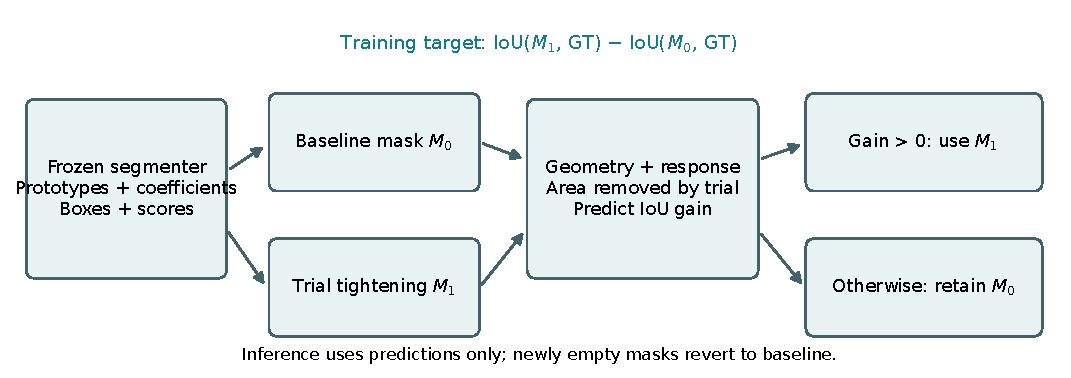
\includegraphics[width=.98\textwidth]{method.pdf}
\caption{Response-conditioned calibration. The trial reuses frozen logits and original boxes. Ground truth supervises the offline benefit regressor; deployment uses mask geometry and trial response. Newly empty masks retain their baseline output. Schematic drawn with Matplotlib using code assisted by OpenAI Codex (GPT-6).}
\label{fig:method}
\end{figure*}

\subsection{Geometry and trial-response features}
The gate uses five features: $\log(1+A)$; log elongation of the baseline-mask bounding rectangle; foreground area divided by that rectangle's area; log perimeter-based compactness; and the removed foreground fraction
\begin{equation}
 r=\frac{A-|M^t|}{\max(A,1)}.\label{eq:response}
\end{equation}
The first three geometry quantities use original-image masks. Compactness uses the input-grid binary mask, with four-connected perimeter $p_4$ and area $a$: $\log(1+p_4^2/(4\pi\max(a,1)))$. No category, confidence, GT-derived size, or crowding score enters the gate. The response feature describes what the intervention would do, rather than only what the current mask looks like.

We compare area-only (one feature), shape (four features), and response (all five) regressors. All use histogram gradient boosting with squared loss, 100 boosting iterations, learning rate 0.05, maximum seven leaves, minimum leaf size 80, $L_2$ regularization 1, no early stopping, and seed 20260915. Only the small regressor is fitted; the segmenter remains frozen.

\section{Experimental protocol}
\subsection{Data and evaluation units}
COCO \citep{lin2014coco} train2017 IDs are sorted, shuffled with seed 20260915, and the first 2,000 are retained. The first 1,500 images fit the gates, yielding 10,288 matched slots from 1,486 images. The remaining 500 select among the three gates and a global threshold grid $\{0,0.25,0.5,0.75,1\}$. The response gate and global threshold 0.25 win their respective comparisons. The gate decision threshold remains zero, without a separate search.

Evaluation uses sorted val2017 IDs at positions 500--4999 (zero-based): 4,500 images and 32,831 ordinary GT instances, without density filtering. The first 500 validation images were used in earlier readout development. Fitting and selection images are disjoint from validation, but belong to the segmenter's pretraining dataset. Moreover, validation predictions informed earlier exploration; the final results are frozen-rule confirmation, not a previously unseen blind benchmark. The final gate parameters are fixed before their 4,500-image evaluation.

We decode original COCO annotations with the official tools \citep{cocoeval}; multiple polygons belonging to an annotation remain one instance. Segmentation COCOeval retains crowd handling and its default evaluation limits. We report AP, AP$_{75}$, size-specific AP, and small-object AR on the 0--100 scale. All twelve COCO metrics appear in the supplement.

For a separate fixed-slot diagnostic, predictions are processed in descending confidence. Each nonempty baseline prediction is greedily matched to the best available same-class ordinary GT with box IoU $\geq0.50$. Matches stay fixed across readout variants. Fixed-slot R75 counts mask IoU $\geq0.75$ and divides by \emph{all} ordinary GT, including unmatched instances. A repair crosses from below 0.75 to at least 0.75; damage crosses in the reverse direction. This is distinct from official COCO AR and does not replace mask-based COCO matching. Paired image bootstrap intervals use 2,000 resamples of complete images; they quantify R75 differences, not AP uncertainty.

\subsection{Frozen decoder and controls}
We use Ultralytics 8.4.100 COCO-pretrained YOLO26m-seg, with the one-to-one inference branch, image size 640, confidence cutoff 0.001, maximum 300 candidates, FP32, batch size one, and non-retina masks. Export follows the selected utilities: upsample logits, crop on the input grid, binarize, then scale binary masks to the original image and cast to bytes. The baseline is checked against this mask-decoding path; we do not equate the experiment with a full reproduction of a published \texttt{model.val} result.

The gate and boundary-only controls preserve every baseline nonempty candidate and its box, class, and score. Fixed smooth applies the trial to all candidates and drops newly empty exports. Filtering-only drops those same candidates but retains baseline masks; boundary-only changes masks while restoring newly empty ones. Their factorial comparison separates the two effects. Area and shape gates test whether trial response adds value beyond geometry. A global threshold selected on train2017 supplies a tuned scalar control.

Finally, the m-fitted gates transfer unchanged to COCO-pretrained YOLO26s-seg on the same 4,500 images. No s-model annotations are used for refitting or selection. This tests transfer across model scales within one architecture family, not cross-dataset or cross-architecture generalization.

OpenAI Codex (GPT-6) assisted protocol development, Python implementation, and visualization code under researcher direction. Tables and plots are generated programmatically from archived model outputs and evaluation summaries; the accompanying sources document the computational steps.

\section{Results}
\subsection{Normal-mask performance}
Table~\ref{tab:main} reports normal-box COCO results. RCMC raises m-model mask AP from 43.38 to 43.94 (+0.56 points), AP$_{75}$ by 0.78, AP$_S$ by 0.88, and AR$_S$ by 1.58. AP$_L$ changes by $-0.01$. Frozen s transfer gives +0.47 AP, +0.51 AP$_{75}$, +0.70 AP$_S$, and +1.32 AR$_S$. These are modest aggregate improvements, with larger changes on small objects. They are obtained without expanding boxes or adjusting confidence ranking.

The full gate exceeds the selected global threshold by 0.33 AP on m and 0.23 on s. Its additional gain over fixed smooth is smaller: 0.11 and 0.10 AP. Area-only and shape gates also improve the baseline, but their point estimates remain below the response gate. We do not attach AP significance claims to these differences because the available bootstrap analysis concerns fixed-slot R75.

\begin{table*}[!t]
\caption{COCO segmentation metrics on 4,500 val2017 images. All values are on the 0--100 scale. Gates are fitted using m-model train2017 predictions; s results use the same frozen gates. Bold identifies the proposed method, not necessarily the best value in each column.}
\label{tab:main}\centering\small
\begin{tabular}{lrrrrrr}
\toprule Readout & AP & AP$_{75}$ & AP$_S$ & AP$_M$ & AP$_L$ & AR$_S$\\\midrule
\tableinput{tables/main_results.tex}
\end{tabular}
\end{table*}

\subsection{The repair--damage trade-off}
Fixed smooth repairs 907 m-model failures but damages 576 initially successful masks. RCMC repairs 801 and damages 445: 106 fewer repairs, 131 fewer damages, and 25 additional net successes. On s, the corresponding change is from 841/556 to 729/389, giving 55 additional net successes. Thus the relative reduction in damage is 22.74\% and 30.04\%, respectively. The gate retains some harmful operations; its benefit is a changed balance, not elimination of damage (Fig.~\ref{fig:transitions}).

\begin{figure*}[!t]
\centering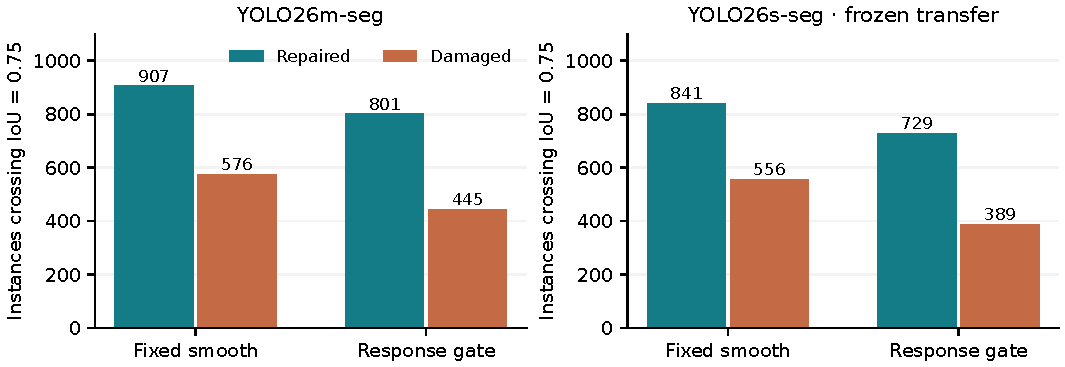
\includegraphics[width=.98\textwidth]{repair_damage.pdf}
\caption{Transitions at fixed-slot mask IoU 0.75. Calibration is applied with frozen candidate identities. The response gate retains fewer successful corrections than fixed smooth, but avoids more harmful corrections: net gains increase from 331 to 356 (m) and from 285 to 340 (s).}
\label{fig:transitions}
\end{figure*}

\begin{table}[!t]
\caption{Fixed-slot transitions. $\Delta$R75 is in percentage points and includes all 32,831 ordinary GT in the denominator.}
\label{tab:transitions}\centering\small
\setlength{\tabcolsep}{3pt}
\begin{tabular}{llrrrr}
\toprule Model & Rule & Repair & Damage & Net & $\Delta$R75\\\midrule
\tableinput{tables/transitions.tex}
\bottomrule
\end{tabular}
\end{table}

Fixed-slot R75 changes from 58.07\% to 59.15\% on m and from 53.09\% to 54.13\% on s (Table~\ref{tab:transitions}). The m gate exceeds fixed smooth by 0.076 points, with a 95\% paired interval of $[-0.018,0.169]$. The s difference is 0.168 points, with interval $[0.070,0.270]$. Against the area gate, the differences are 0.302 points $[0.183,0.424]$ and 0.305 points $[0.188,0.417]$. The evidence for an advantage over uniform smoothing is therefore stronger on s under this diagnostic; m does not show a decisive R75 difference from that comparator.

\subsection{Does trial response help identify harmful edits?}
Table~\ref{tab:decisions} groups matched m-model instances by each gate's decision and measures the actual trial IoU change. The area gate rejects a group whose mean change is still positive. The response gate rejects 2,847 slots with a mean change of $-0.0250$, while its 27,579 accepted slots have a positive mean change of 0.0053. This supports using response to distinguish the expected benefit of the action beyond size alone. The rejection is imperfect: 39.66\% of rejected slots would improve in continuous IoU. These descriptive group means explain selective abstention, not per-instance correctness guarantees.

\begin{table}[!t]
\caption{Actual trial IoU change in matched m-model decision groups, multiplied by 100. The gates are frozen before these measurements.}
\label{tab:decisions}\centering\small
\begin{tabular}{lrr}
\toprule Gate & Accepted group & Rejected group\\\midrule
\tableinput{tables/decision_groups.tex}
\bottomrule\end{tabular}
\end{table}

\subsection{Which failure objects improve?}
The high-coverage failure group contains 1,701 m-model and 1,596 s-model slots. RCMC repairs 457 (26.87\%) and 402 (25.19\%) of them. Table~\ref{tab:failure} shows higher mean IoU and purity, accompanied by lower coverage. For m, purity rises from 66.30\% to 70.64\%, while coverage decreases from 98.07\% to 96.45\%. This is consistent with removing enough false-positive pixels to compensate for lost true positives, rather than preserving every target pixel.

\begin{table}[!t]
\caption{Annotation-defined high-coverage failures: box IoU $\geq0.75$, baseline coverage $\geq0.95$, baseline mask IoU $<0.75$. Group sizes are 1,701 (m) and 1,596 (s). Purity and coverage are percentages. Crossings are count (group repair percentage). These conditional repair rates are not overall AP gains.}
\label{tab:failure}\centering\small
\setlength{\tabcolsep}{2pt}
\begin{tabular}{llrrrr}
\toprule Model & Readout & IoU & Purity & Coverage & Crossings\\\midrule
\tableinput{tables/failure_group.tex}
\bottomrule
\end{tabular}
\end{table}

Uniform tightening repairs more members of this selected failure group: 511 and 447. Because every group member initially fails, this table cannot measure damage to successful instances. The broader transition table is essential: RCMC trades some group repair for fewer losses elsewhere. Nor does this group identify all repairable masks; the m gate also repairs 344 of the 9,660 other matched failures.

\subsection{Isolation and computational cost}
For m, filtering-only changes AP by +0.000901 points, boundary-only by +0.448457, and their combination by +0.449391. The interaction is +0.000033 points. This controlled decomposition attributes nearly all of the fixed intervention's AP gain to changed masks rather than dropping newly empty predictions. The final gate restores such predictions and preserves the baseline's 506,966 nonempty candidate exports.

The practical cost is material (Table~\ref{tab:latency}). On an RTX 4060 Laptop GPU, mean latency is 37.26 ms for the official predictor, 35.60 ms for the chunked fixed-smooth implementation, and 57.37 ms for the response gate. The measurement includes preprocessing, forward computation, mask work, feature transfer, and CPU tree prediction; it excludes disk I/O, initialization, and COCO scoring. The 80-image, four-round, batch-one measurement includes 320 timed calls per variant. Different chunking and the first official timing block affect comparisons, so the lower fixed-rule latency is not evidence that adding an operation inherently speeds up the model. The response gate costs 21.77 ms more than fixed smooth under this setup.

\begin{table}[!t]
\caption{Batch-one FP32 latency on RTX 4060 Laptop GPU. All gate overhead is included; this is not TensorRT latency.}
\label{tab:latency}\centering\small
\begin{tabular}{lrrr}
\toprule Variant & Mean ms & Median ms & P95 ms\\\midrule
\tableinput{tables/latency.tex}
\bottomrule
\end{tabular}
\end{table}

\section{Discussion and limitations}
The experiments identify a correctable \emph{readout} failure. Some existing response maps admit better masks under a stricter threshold, and a trial-response feature helps decide which corrections to retain. This does not prove that the default threshold is globally wrong, that the prototypes are optimal, or that coefficient similarity causes the failure. The same intervention is harmful for hundreds of initially correct predictions. Eq.~\ref{eq:condition} explains why removal alone cannot guarantee improved segmentation.

The scope is also limited by the available evidence. Results concern 4,500 validation images, two scales of one model family, one calibration split, and one fitted gate per feature set. The validation set had been explored previously. We provide no test-dev claim, independent-data replication, repeated-split stability estimate, or AP confidence interval. No direct comparison against retrained PointRend or BPR is included; our controlled comparisons measure selection within a fixed readout action space.

Supervision covers matched ordinary instances, whereas inference applies the gate to unmatched candidates as well. COCO AP includes these predictions, but the fixed-slot diagnostic does not establish a benefit for their population separately. In addition, threshold tightening cannot generate a missing candidate or reconstruct foreground absent from the baseline mask. The observed purity gain can coexist with reduced coverage, and small negative changes remain on large-object m metrics. Finally, the current feature extraction adds substantial latency; its engineering cost must be considered alongside the extra 0.10--0.11 AP over the simple fixed rule.

\section{Conclusion}
Response-conditioned mask calibration uses the effect of a trial tightening to predict whether a frozen instance mask should be changed. The diagnosis separates boundary correction from candidate filtering and exposes both repairs and damage. A compact supervised gate improves normal-box COCO results and transfers across YOLO26 scales, while reducing the damage caused by uniform tightening. The evidence supports selective use of existing mask response, with bounded accuracy gains and explicit computational cost. It motivates further work on richer corrective actions and cheaper benefit estimation without attributing all segmentation failures to a single upstream mechanism.

\section*{Declaration of generative AI use}
OpenAI Codex (GPT-6) assisted literature checking, manuscript organization, drafting, code development, and figure preparation. This preparation copy awaits the authors' final review and responsibility declaration before any submission.

\bibliographystyle{elsarticle-harv}
\bibliography{references}
\end{document}
